% Template adapted from that for Scribe Notes - CS500 (Spring 2016)
% (template is a modified version of one prepared by Erik Demaine at MIT)
%
\documentclass[11pt]{article}
\usepackage{latexsym}
\usepackage{amsmath}
\usepackage{amssymb}
\usepackage{amsthm}
\usepackage{amsfonts}
\usepackage{epsfig}
%\usepackage{psfig}
\usepackage{enumerate}  % use this for lettered points
\usepackage{hyperref}   % to add links

\newcommand{\handout}[5]{
  \noindent
  \begin{center}
  \framebox{
    \vbox{
      \hbox to 5.78in { \textbf{PHYS 447} \hfill #2 }
      \vspace{4mm}
      \hbox to 5.78in { {\Large \hfill #5  \hfill} }
      \vspace{2mm}
      \hbox to 5.78in { \emph{#3 \hfill #4} }
    }
  }
  \end{center}
  \vspace*{4mm}
}

\newcommand{\lecture}[4]{\handout{#1}{#2}{#3}{-: #4}{#1}}
\newcommand{\R}{\mathbb{R}}     % use for capital R real number set symbol
\newcommand{\Z}{\mathbb{Z}}     % use for capital Z integer set symbol
\newcommand{\D}[2][]{\frac{\partial#1}{\partial#2}}
% tabbing environment for pseudo-code 
\newenvironment{code} {
\begin{tt}
\begin{tabbing}
\ \ \ \ \= \ \ \ \ \= \ \ \ \ \= \ \ \ \ \= \ \ \ \ \= \ \ \ \ \=  \ \ \ \ \= \ \ \ \ \= \\ \kill
}{
\end{tabbing}
\end{tt}
}

\newtheorem{theorem}{Theorem}
\newtheorem{corollary}[theorem]{Corollary}
\newtheorem{lemma}[theorem]{Lemma}
\newtheorem{observation}[theorem]{Observation}
\newtheorem{proposition}[theorem]{Proposition}
\newtheorem{definition}[theorem]{Definition}
\newtheorem{claim}[theorem]{Claim}
\newtheorem{fact}[theorem]{Fact}
\newtheorem{assumption}[theorem]{Assumption}

% 1-inch margins, from fullpage.sty by H.Partl, Version 2, Dec. 15, 1988.
\topmargin 0pt
\advance \topmargin by -\headheight
\advance \topmargin by -\headsep
\textheight 8.9in
\oddsidemargin 0pt
\evensidemargin \oddsidemargin
\marginparwidth 0.5in
\textwidth 6.5in

\parindent 0in
\parskip 1.5ex
%\renewcommand{\baselinestretch}{1.25}

\begin{document}
\lecture{Computational fluid dynamics}{Spring 2016}{}{}
% =========================================================================== %
\section{Introduction}

\vspace{1cm}
This intent of this project was to learn about the physics of fluids and
observe the behaviour in computer simulations.
The process was carried out by starting with simplifying assumptions on the
model, choosing a discretization method, then writing code in Python. At each
following step, an assumption would be generalized so that the change could be
observed. The equations were examined in 1-dimension first so an example will
be shown before the transition to 2-dimensions.

Fluid flow equations addressed:
\begin{itemize}\itemsep0em 
\item linear convection
\item nonlinear convection
\item diffusion
\item Burgers equation (convection with diffusion)
\item Navier-Stokes (cavity flow and channel flow conditions)
\end{itemize}


\section{Physics}

The equations governing models of flow are described in this section.

\subsection{Introduction to models in 1-dimensional form}
Beginning with 1-dimensional models, we can describe the differences
between the behaviours of the systems dictated by these equations. They
have their analogues in 2-dimensions.

Starting off, the simplest model looked at was the 1-dimensional equation
describing convective flow without diffusion. It describes the propagation
of a wave with constant speed $c$. There is no deformation of shape of the
initial condition's wave as it propagates. \ref{1d_linconv}

In the nonlinear case, the constant speed is replaced by $u$ which is the
solution $u(x,t)=u_0(x-ct)$ given an initial condition $u(x,0)=u_0(x)$
The speed of propagation is different depending upon the location.
Because of this, shocks may be observed (see corresponding treatment in the
numerical considerations section \ref{}). It is also known as the inviscid
Burgers equation.
\ref{1d_nonlinconv}

Then diffusion is considered without any convection.
If $u$ is temperature, then this is the heat equation.
It is governed by a second-order partial derivative. \ref{1d_diffusion}

For the last of the equations with time evolution, nonlinear convection
and diffusion are treated simultaneously. Since viscosity is now accounted
for with the diffusion term, this is the general Burgers equation. It has
applications outside of fluid dynamics, for example in acoustics.
\ref{1d_Burgers}

\begin{align}
& \text{linear convection} &
\frac{\partial u}{\partial t} + c \frac{\partial u}{\partial x} &= 0		\label{1d_linconv}
\\ \nonumber \\ & \text{(inviscid Burgers) nonlinear convection} &
\frac{\partial u}{\partial t} + u \frac{\partial u}{\partial x} &= 0		\label{1d_nonlinconv}
\\ \nonumber \\ & \text{linear diffusion} &
\frac{\partial u}{\partial t} &= \nu \frac{\partial^2 u}{\partial x^2}		\label{1d_diffusion}
\\ \nonumber \\ & \text{Burgers' equation} &
\frac{\partial u}{\partial t} + u \frac{\partial u}{\partial x} &= \nu \frac{\partial^2 u}{\partial x^2}	\label{1d_Burgers}
\end{align}

% this is useful for spacing equations when they're too far apart... or something
\hspace{1cm}
% equation stuff
%\begin{align*}
%\end{align*}

\subsection{Extension to 2-dimensional models}
The expressions introduced in their 1-dimensional form are now shown
extended to two dimensions.
\subsubsection{Linear convection (2d)}
The conversion from one- to two-dimensions is straightforward for linear
convection. As two spatial components are changing, it is sufficient to
duplicate the original spatial variation in the new dimension.
\begin{align}
\frac{\partial u}{\partial t} + c\left(\frac{\partial u}{\partial x}  + \frac{\partial u}{\partial x} \right)
&= 0		\label{2d_linconv}
\end{align}

\subsubsection{Nonlinear convection (2d)}
Nonlinear in an extra dimension requires a different treatment.
The constant velocity is now a vector-valued velocity with two dimensions
$(u, v)$, with partial derivatives, we now have coupled equations.

\begin{align}
\frac{\partial u}{\partial t} + u\frac{\partial u}{\partial x}  + v\frac{\partial u}{\partial y} 
&= 0		\nonumber \\ \nonumber\\
\frac{\partial v}{\partial t} + u\frac{\partial v}{\partial x}  + v\frac{\partial v}{\partial y} 
&= 0
	\label{2d_nonlinconv}
\end{align}

\subsubsection{Diffusion (2d)}
Diffusion affects flow equally in both components in two dimensions, so
again, a duplication in the y-component works.
\begin{align}
\frac{\partial u}{\partial t} &= \nu \left(\frac{\partial^2 u}{\partial x^2} + \frac{\partial^2 u}{\partial y^2}\right)		\label{2d_diffusion}
\end{align}

\subsubsection{Burgers (2d)}
As in the case with nonlinear convection, coupled PDEs are required to
describe the system. The two independent variables $u$, and $v$ are coupled
in this system to form a vector field.

\begin{align}
\frac{\partial u}{\partial t} + u \frac{\partial u}{\partial x} + v \frac{\partial u}{\partial y}
&= \nu \left(\frac{\partial^2 u}{\partial x^2} + \frac{\partial^2 u}{\partial y^2}\right)
\nonumber \\ \nonumber \\
\frac{\partial v}{\partial t} + u \frac{\partial v}{\partial x} + v \frac{\partial v}{\partial y}
&= \nu \left(\frac{\partial^2 v}{\partial x^2} + \frac{\partial^2 v}{\partial y^2}\right)	\label{2d_Burgers}
\end{align}

\subsubsection{Navier-Stokes for incompressible fluid}

Velocity and pressure need to be included and each affects the other.

We need to involve the continuity equation for fluid with constant density
$\rho$ (mass conservation) and the vector equation for conservation of
momentum, which depends upon $\rho$. Equation (\ref{continuity}) acts as
a constraint to the equation of motion (\ref{consmom}).

For compressible flows, we are able to relate pressure and density, but
since we are dealing with the incompressible version, we have no such
equation of state. A different way of coupling the equations is required.

\begin{align}
&\text{continuity equation (conservation of mass)}
	&\nabla \cdot \vec{u} &= 0	\label{continuity}
	\\ \nonumber \\
&\text{conservation of momentum}
	&\frac{\partial \vec{u}}{\partial t} + (\vec{u} \cdot \nabla) \vec{u}
	&= -\frac{1}{\rho} \nabla p + \nu \nabla ^2 \vec{u}
\label{consmom}
\end{align}
 
Componentwise, the equations become:
\begin{align}
&\text{conservation of mass}
	&\frac{\partial u}{\partial x} + \frac{\partial v}{\partial y} &= 0
	\label{component_consmass}
	\\ \nonumber \\
&\text{conservation of momentum}
	\label{component-1_consmom}
	&\frac{\partial u}{\partial t} + u\frac{\partial u}{\partial x} + v\frac{\partial u}{\partial y}
	&= -\frac{1}{\rho} \frac{\partial p}{\partial x} 
	+ \nu \left(\frac{\partial^2 u}{\partial x^2} + \frac{\partial^2 u}{\partial y^2}\right)
	\\ \nonumber \\
	&
	&\frac{\partial v}{\partial t} + u\frac{\partial v}{\partial x} + v\frac{\partial v}{\partial y}
	&= -\frac{1}{\rho} \frac{\partial p}{\partial y} 
	+ \nu \left(\frac{\partial^2 v}{\partial x^2} + \frac{\partial^2 v}{\partial y^2}\right)	
	\label{component-2_consmom}
\end{align}

The equations retain the same form: in conservation of momentum, the first term is the
steady partial, the second and third are associated with convection,
the final term is the viscous term multiplying the Laplacian of that
component velocity and is associated with diffusion.

By taking derivatives of expressions\ref{component-1_consmom} and \ref{component-2_consmom},
we obtain the divergence of the momentum. That is, adding $\frac{\partial }{\partial x}$
(\ref{component-1_consmom}) and $\frac{\partial }{\partial y}$ (\ref{component-2_consmom}),
we have, term by term:

\begin{align}
\frac{\partial}{\partial t} \left( \frac{\partial u}{\partial x} \right) &
	\nonumber \\ \nonumber \\
+ \frac{\partial u}{\partial x} \frac{\partial u}{\partial x}
 + u \frac{\partial^2 u}{\partial x^2}	 &
	\nonumber \\ \nonumber \\
+ \frac{\partial v}{\partial x} \frac{\partial u}{\partial y}
 + v \frac{\partial^2 u}{\partial x \partial y}
 	\nonumber \\ \nonumber \\
& = -\frac{1}{\rho} \frac{\partial^2 p}{\partial x^2}
	\nonumber \\ \nonumber \\
& + \nu \left( \D[^3u]{x^3} + \D{x} \D[^2u]{y^2} \right)
	\nonumber % \\
\end{align}
%	\nonumber
%	\\
%\text{add to similar treatment of partial with respect to y on (\ref{component-2_consmom}):}
%	\nonumber \\ \nonumber
%\\
add to similar treatment of partial with respect to $y$ on (\ref{component-2_consmom}):
\begin{align}
\D{t} \D[v]{y} + \D[u]{y}\D[u]{x} + u \D{y}\D[v]{x} + \D[v]{y}\D[v]{y} + v \D[^2 v]{y^2}
& = -\frac{1}{\rho} \frac{\partial^2 p}{\partial y^2}
 + \nu \left( \D{y} \D[^2v]{x^2} + \D[^3v]{y^3} \right)
	\nonumber \\ \nonumber
\end{align}
the left-hand side becomes
\begin{align}
&\D{t} \left( \D[u]{x} + \D[v]{y} \right)
	+ \D[u]{x}\D[u]{x} + \D[u]{y}\D[u]{x}
	+ u \left( \D[^2u]{x^2} + \D{y}\D[v]{x} \right)
	+ \D[v]{x}\D[u]{y} + \D[v]{y}\D[v]{y}
	+ v \left( \D[^2u]{x^2} + \D[^2v]{y^2} \right)
	\nonumber \\ \nonumber
= &\D{t} \left( \D[u]{x} + \D[v]{y} \right)
	+ \D[u]{x}\D[u]{x} + \D[u]{y}\D[u]{x}
	+ u \D{x} \left( \D[u]{x} + \D[v]{y} \right)
	+ \D[v]{x}\D[u]{y} + \D[v]{y}\D[v]{y}
	+ v \D{y} \left( \D[u]{x} + \D[v]{y} \right)
\end{align}
looking at the common terms in parentheses (divergence of velocity),
we know these = 0 from the conservation of mass equation, which we must obey
 (\ref{component_consmass}), so we are left with the remaining terms
\begin{align}
= \D[u]{x}\D[u]{x} + \D[u]{y}\D[u]{x}
	+ \D[v]{x}\D[u]{y} + \D[v]{y}\D[v]{y}
= \left(\D[u]{x}\right)^2 + 2\D[v]{x}\D[u]{y} + \left(\D[v]{y}\right)^2
\label{lhs}
\end{align}
the right-hand side becomes
\begin{align}
-\frac{1}{\rho} \left( \D[^2p]{x^2} + \D[^2p]{y^2} \right)
&+\nu \left( \D[^3u]{x^3} + \D{x} \D[^2u]{y^2} + \D{y} \D[^2v]{x^2} + \D[^3v]{y^3} \right)
	\nonumber \\ \nonumber
= -\frac{1}{\rho} \left( \D[^2p]{x^2} + \D[^2p]{y^2} \right)
&+ \nu \left[
  \D[^2]{x^2} \left( \D[u]{x} + \D[v]{y} \right)
+ \D[^2]{y^2} \left( \D[u]{x} + \D[v]{y} \right)
  \right]
  \label{rhs}
\end{align}
%  \nonumber \\ \nonumber
 \text{again, apply equation (\ref{component_consmass}) to yield}
  \\
\begin{align}
= -\frac{1}{\rho} \left( \D[^2p]{x^2} + \D[^2p]{y^2} \right)
\end{align}
Putting LHS (\ref{lhs}) and RHS (\ref{rhs}) together, we have
\begin{align}
&\left(\D[u]{x}\right)^2 + 2\D[v]{x}\D[u]{y} + \left(\D[v]{y}\right)^2
=
-\frac{1}{\rho} \left( \D[^2p]{x^2} + \D[^2p]{y^2} \right)
\nonumber \\
\text{(re-arrange terms)}~~ \nonumber \\
\Rightarrow~~~&\D[^2p]{x^2} + \D[^2p]{y^2} =
- \rho \left[ \left(\D[u]{x}\right)^2 + 2\D[v]{x}\D[u]{y} + \left(\D[v]{y}\right)^2 \right]
\label{poisson_continuous_2-component} \\
\text{which has form}& \nonumber \\ \nonumber
\Rightarrow~~~&\nabla^2 p = function
\end{align}
This is Poisson's equation for pressure in two dimensions.
Equations (\ref{continuity}) and {\ref{consmom}) are satisfied simultaneously.
This relation between pressure and velocity can be used to couple the equations
for Navier-Stokes. (When RHS is 0, it is the Laplace equation.) $f$ is the
function such that pressure satisfies the Poisson equation.


\section{Numerical schemes and considerations}

In some simpler cases, the discretization of the above continuous equations can
be a straightforward translation. In general, the following differencing schemes are used
for this project:

\begin{itemize}
\item time stepping: forward difference
\item convection: backward difference
\item diffusion: central difference, second order
\end{itemize}

The discretized equations are solved for the values of interest.
The value at the next time step, is dependent upon various values of the current
time step. We start with given initial conditions.

The spatial component is discretized into a grid according to the number of
dimensions and solutions are found for each point over a set number of time
steps, or after a specified tolerance is satisfied indicate steady state having
been reached.

Superscripts $n$ are used for time steps,
and subscripts $i$ and $j$ for spatial grid points.

Solving these equations has some issues that do not arise in the continuous form
and these will be addressed along the way in the examples that follow.

\subsection{Discretization examples (with transposition to solve for next iterative step)}
Simpler examples of discretization will be shown to have the idea before moving
on to more generalized models. However, all of the differencing schemes here are
based on using a Taylor expansion about a point to obtain the definition of the
derivative and in turn we use an approximation to that derivative by disregarding
higher order terms.

\subsubsection{Linear Convection: 1-d to 2-d}
%%%%%%%%%%%%%%%%%%%%%%%%%%%%%%%%%%%%%%%%%%%%%%%%%%%%%%%%%%%%%%%%%%%%%%%%%%%%%%
%%% do I want to do some Taylor expanding here? Nice for my own reference  %%%
%%% but may not be necessary/good for report. Nope: Hit page limit already %%%

With forward difference on the time dependent term and backward difference on the second, Equation (\ref{1d_linconv}) becomes:

\begin{align}
\frac{u^{n+1}_i - u^n_i}{\Delta t} + c \frac{u^n_i - u^n_{i-1}}{\Delta x} = 0
\label{discrete_1d_linconv}
\intertext{Transpose this to get values at time $t_{n+1}$ at position $x_i$.}
u^{n+1}_i = u^{n}_i - \frac{c \Delta t}{\Delta x} (u^n_i - u^n_{i-1})
\end{align}

In two dimensions, we have $x$- and $y$-components.
From (\ref{2d_linconv}) or above (\ref{discrete_1d_linconv}), we get:

\begin{align}
&\frac{u^{n+1}_{i,j} - u^{n}_{i,j}}{\Delta t}
	+ c \frac{u^{n}_{i,j} - u^{n}_{i-1,j}}{\Delta x}
	+ c \frac{u^{n}_{i,j} - u^{n}_{i,j-1}}{\Delta y} = 0 \\
\Rightarrow ~~
&u^{n+1}_{i,j} = u^n_{i,j}
				- \frac{c \Delta t}{\Delta x}(u^n_{i,j} - u^n_{i-1,j})
				- \frac{c \Delta t}{\Delta y}(u^n_{i,j} - u^n_{i,j-1})
\end{align}

The subsequent models will be discretized in their 2-dimensional forms.
But first, it would be helpful to address some constraints in using
differencing methods in numerical schemes.

\subsubsection{Accuracy and the CFL condition}
When using these methods to compute solutions, there are sources of error that
will alter the results. Awareness of these effects will help to interpret the results
correctly. Firstly, there is the error introduced from the discretizations
being derived from approximations. If the grid spacing is wide, these errors will
dominate over the imprecision inherent to the computer architecture and the selected
precision level in the programming language.

If we feed an initial condition of a particular waveform to the linear convection model,
the expected solution would be the same shape waveform in another location after being
convected over time, with speed $u$ without any other effect. However, we do see a shape
change in Figure \ref{fig:num_diff}. The initial condition is a hat function
and as it is convected, it also accumulates round-off error at every iteration. This
numerical diffusion is from the method of computation and not expected in the physics
of the system. The effect can be somewhat mitigated by taking a finer spatial mesh,
as in Figure \ref{fig:num_diff_fine_mesh}.

It would be tempting to take smaller and smaller grid sizes, but a problem arises when
the grid size is smaller than the distance moved by a point on the waveform in one
timestep, i.e. if $u\Delta t > \Delta x$. Non-physical artefacts appear in the computations
plotted in Figure \ref{fig:num_diff_too_fine}.

To prevent this from occurring. The size of the timestep and grid size must be constrained
against each other using

\begin{align}
\sigma = \frac{u \Delta t}{\Delta x} \leq \sigma_{max}
\end{align}

where $\sigma$ is the Courant number and the $u$ is the speed (non-negative).
The constraint is called the Courant-Friedrichs-Lewy or CFL condition.
For explicit methods (as we have here), $\sigma$ should be less than 1.
This will be a consideration for any part of this project where values may change faster
than the timestep is able to show so it will be in effect at any point onward from here.
Adding the condition to decide timesteps based on chosen gridspacing (or vice versa)
will prevent these undesired artefacts from appearing.

\subsubsection{Nonlinear convection}
As with equations in (\ref{2d_nonlinconv}), we need to handle non-constant velocity
fields $u$ and $v$.

\begin{align}
&\frac{u^{n+1}_{i,j} - u^{n}_{i,j}}{\Delta t}
	+ u^n_{i,j} \frac{u^{n}_{i,j} - u^{n}_{i-1,j}}{\Delta x}
	+ v^n_{i,j} \frac{u^{n}_{i,j} - u^{n}_{i,j-1}}{\Delta y} = 0	\nonumber \\
&\frac{v^{n+1}_{i,j} - v^{n}_{i,j}}{\Delta t}
	+ u^n_{i,j} \frac{v^{n}_{i,j} - v^{n}_{i-1,j}}{\Delta x}
	+ v^n_{i,j} \frac{v^{n}_{i,j} - v^{n}_{i,j-1}}{\Delta y} = 0 \\
\Rightarrow ~~ \nonumber \\
&u^{n+1}_{i,j} = u^n_{i,j}
				- \frac{u^n_{i,j} \Delta t}{\Delta x}(u^n_{i,j} - u^n_{i-1,j})
				- \frac{v^n_{i,j} \Delta t}{\Delta y}(u^n_{i,j} - u^n_{i,j-1})
																 \nonumber \\
&v^{n+1}_{i,j} = v^n_{i,j}
				- \frac{u^n_{i,j} \Delta t}{\Delta x}(v^n_{i,j} - v^n_{i-1,j})
				- \frac{v^n_{i,j} \Delta t}{\Delta y}(v^n_{i,j} - v^n_{i,j-1})
\end{align}

\subsubsection{Diffusion}
This is diffusion without convection from equation (\ref{2d_diffusion}).
This has second-order partial derivatives in the spatial components so a second-order
scheme will be used. A central difference is appropriate to the isotropic nature of
diffusion; the value at a particular point is subjected to the numerical influence of
its neighbours in a manner that is independent of which direct the neighbour is.

%%%%%%%%%%%%%%%%%%%%%%%%%%%%%%%%%%%%%%%%%%%%%%%%%%%%%%%%%%%%%%%%%%%%%%%%%%%%
%%% derive second order scheme here? Nope. Hitting the page limit already%%%

So the discretization becomes:

\begin{align}
&\frac{u^{n+1}_{i,j} - u^{n}_{i,j}}{\Delta t} = \nu
	\left( \frac{u^n_{i+1,j} - 2u^n_{i,j} + u^n_{i-1,j}}{\Delta x^2} \right.
  + \left. \frac{u^n_{i,j+1} - 2u^n_{i,j} + u^n_{i,j-1}}{\Delta y^2} \right)		\\
\Rightarrow~~
&u^{n+1}_{i,j} = u^n_{i,j}
			+ \frac{\nu \Delta t}{\Delta x} (u^n_{i+1,j} - 2u^n_{i,j} + u^n_{i-1,j})
			+ \frac{\nu \Delta t}{\Delta y} (u^n_{i,j+1} - 2u^n_{i,j} + u^n_{i,j-1})
\end{align}

\subsubsection{Burgers' Equation}
This handles nonlinear convective flow with diffusion simultaneously. Discretizing
from equations (\ref{2d_Burgers}) goes as expected from the the previous steps.

\begin{align}
&\frac{u^{n+1}_{i,j} - u^{n}_{i,j}}{\Delta t}
	+ u^n_{i,j} \frac{u^{n}_{i,j} - u^{n}_{i-1,j}}{\Delta x}
	+ v^n_{i,j} \frac{u^{n}_{i,j} - u^{n}_{i,j-1}}{\Delta y}
=\nu	\left( \frac{u^n_{i+1,j} - 2u^n_{i,j} + u^n_{i-1,j}}{\Delta x^2} \right.
  + \left. \frac{u^n_{i,j+1} - 2u^n_{i,j} + u^n_{i,j-1}}{\Delta y^2} \right)	
																	\nonumber \\
&\frac{v^{n+1}_{i,j} - v^{n}_{i,j}}{\Delta t}
	+ u^n_{i,j} \frac{v^{n}_{i,j} - v^{n}_{i-1,j}}{\Delta x}
	+ v^n_{i,j} \frac{v^{n}_{i,j} - v^{n}_{i,j-1}}{\Delta y}
=\nu
	\left( \frac{v^n_{i+1,j} - 2v^n_{i,j} + v^n_{i-1,j}}{\Delta x^2} \right.
  + \left. \frac{v^n_{i,j+1} - 2v^n_{i,j} + v^n_{i,j-1}}{\Delta y^2} \right)	
																		 \\
\Rightarrow ~~ \nonumber \\
u^{n+1}_{i,j}
	&= u^n_{i,j}
	- \frac{u^n_{i,j} \Delta t}{\Delta x}(u^n_{i,j} - u^n_{i-1,j})
	- \frac{v^n_{i,j} \Delta t}{\Delta y}(u^n_{i,j} - u^n_{i,j-1})
	+\nu \Delta t \left( \frac{u^n_{i+1,j} - 2u^n_{i,j} + u^n_{i-1,j}}{\Delta x^2} \right.
	            + \left. \frac{u^n_{i,j+1} - 2u^n_{i,j} + u^n_{i,j-1}}{\Delta y^2} \right)	
																 \nonumber \\
v^{n+1}_{i,j}
	&= v^n_{i,j}
	- \frac{u^n_{i,j} \Delta t}{\Delta x}(v^n_{i,j} - v^n_{i-1,j})
	- \frac{v^n_{i,j} \Delta t}{\Delta y}(v^n_{i,j} - v^n_{i,j-1})
	+\nu \Delta t \left( \frac{v^n_{i+1,j} - 2v^n_{i,j} + v^n_{i-1,j}}{\Delta x^2} \right.
			   + \left. \frac{v^n_{i,j+1} - 2v^n_{i,j} + v^n_{i,j-1}}{\Delta y^2} \right)	
\end{align}

\subsection{Navier-Stokes}
At this point, some of the expressions that we have in the continuous case do not work so well
when directly translated to discretized form for our numerical computations.
We will see that in trying to iteratively solve a discretized Poisson equation, while we would
like to have a divergence-free velocity,
due to numerical effects, it may not always equal zero at each iteration. The strategy used
here will be to calculate what the conservation of momentum equation should be at the next step
but then before considering the step complete, do an intermediate calculation for the divergence
being zero, thereby preserving continuity (conservation of mass), and only then complete that
iteration.

\subsubsection{Discretizing the momentum equation}
First, we examine how the problem of non-zero divergence of velocity may arise when we
discretize the equation of motion (\ref{consmom}) keeping it in vector form.

\begin{align}
& \frac{\vec{u}^{n+1} - \vec{u^n}}{\Delta t} + \vec{u}^n \cdot \nabla \vec{u}^n
 = -\frac{1}{\rho} \nabla p + \nu \nabla^2 \vec{u}^n \nonumber \\
\Rightarrow ~~&
\vec{u}^{n+1} = \vec{u}^n + \Delta t \left[ -\vec{u}^n \cdot \nabla \vec{u}^n
			  - \frac{1}{\rho} \nabla p - \nu \nabla^2 \vec{u}^n \right]
\label{discrete_mom}
\end{align}

Following similar steps as in the continuous case, we take the divergence,
here $\nabla \cdot$(\ref{discrete_mom}).

\begin{align}
\nabla \cdot \vec{u}^{n+1} = \nabla \cdot \vec{u}^n
 + \Delta t \left[ -\nabla \cdot \vec{u}^n \cdot \nabla \vec{u}^n
			      - \frac{1}{\rho} \nabla^2 p - \nu \nabla (\nabla^2 \cdot \vec{u}^n) \right]
\label{diverged_mom}
\end{align}
%%%%%%%%%%%% proofread, this still feels weird %%%%%%%%%%%%%%%%%%%%%%%%%
To satisfy continuity (\ref{continuity}), the divergence of the velocity (vector) should
be zero, that is, $\nabla \cdot \vec{u}^{n+1}=0$, however it is possible that $\nabla \cdot \vec{u}^n \neq 0$ due to numerical errors during computation of the velocity field for
Navier-Stokes during the previous step. Because of this, the discretized version cannot simply
have $\nabla \cdot \vec{u}^n$ cancelled out at every occurrence above as we did for the
non-discretized case. So compute pressure such that (\ref{continuity}) is satisfied.
Then use that intermediate step's velocity field solution in the Poisson equation.
The momentum equation and the Poisson equation are both solved within one iterative step.
When solving Poisson, force divergence to be zero in order to have a corrected value for
velocity, then use that vakue for the momentum. Alternating between the two approximates
simultaneous satisfaction of both equations.

\subsubsection{Solving discrete Poisson}
Recall that Poisson has the form (\ref{poisson}), so rearrange (\ref{diverged_mom})
accordingly (with its LHS=0 since we must have that $\vec{u}^{n+1} = 0$ for continuity
to be satisfied).

\begin{align}
& \frac{- \nabla \cdot \vec{u}^n}{\Delta t}
	= - \nabla \cdot (\vec{u}^n \cdot \nabla \vec{u}^n)
	  - \frac{1}{\rho} \nabla^2 p
	  - \nu \nabla^2(\nabla \vec{u}^n)
														  \nonumber \\ \nonumber \\
\Rightarrow ~~&
\nabla^2 p = -\rho \left[
					\frac{ - \nabla \cdot \vec{u}^n}{\Delta t}
					+ \nabla \cdot (\vec{u}^n \cdot \nabla \vec{u}^n)
					+ \nu \nabla^2(\nabla \cdot \vec{u}^n)			\right]
\label{discrete_poisson_vector}
\end{align}

This is the equation that needs to be solved next.

To aid in developing a numerical setup for complete Navier-Stokes, we start with some simpler
cases to build up smaller pieces of code. We begin with Laplace's equation and progress to
Poisson.

\subsubsection{Laplace}
Start with Laplace for the purpose of computational stepping. This will be a simplified form
that will help to build up to the full forms required for computation.

The Laplace equation shows a steady state of a system given boundary
conditions. There is no time parameter. It is the Poisson equation without a source term (RHS = 0).
\begin{align}
\frac{\partial^2 p}{\partial x^2} + \frac{\partial^2 p}{\partial y} &= 0
\label{laplace}
\end{align}

This is discretized using second-order central differencing. As the Laplace operator here
has an effect like that of diffusion, in that it is isotropic. A central differencing scheme
is appropriate since it matches the underlying physics. Over the entire grid of solutions,
each point is solved using contributions from the nearest neighbours in the x and y directions.
This is a five-point stencil used to obtain the solution for that central point. Calculations
are repeated for every point on the grid.

These pressure values $p$ (for the entire grid) all happen
at "false time-step" $n$. There is no time-step, but we do solve by iteratively solving at $n$
every time. The "time" superscript seen in the discretizations for the previous models will be
omitted for these terms since they would all be $n$.

\begin{align}
\frac{p_{i+1,j} - 2p_{i,j} + p_{i-1,j}}{\Delta x^2}
 + \frac{p_{i,j+1} - 2p_{i,j} + p_{i,j-1}}{\Delta y^2} = 0
\label{discrete_laplace}
\end{align}

The next step is to isolate $p_{i,j}$, the value solved on each iteration.
\begin{align}
&\Delta y^2 (p_{i+1,j} - 2p_{i,j} + p_{i-1,j}) + \Delta x^2 (p_{i,j+1} - 2p_{i,j} + p_{i,j-1}) = 0
	\nonumber \\ \nonumber \\
\Rightarrow ~~&
\Delta y^2 (p_{i+1,j} + p_{i-1,j}) + \Delta x^2 (p_{i,j+1} + p_{i,j-1})
 = 2p_{i,j} (\Delta x^2 + \Delta y^2)
	\nonumber \\ \nonumber \\
\Rightarrow ~~&
p_{i,j} = \frac{\Delta y^2 (p_{i+1,j} + p_{i-1,j}) + \Delta x^2 (p_{i,j+1} + p_{i,j-1})}
			 {2(\Delta x^2 + \Delta y^2)}
	\\ \nonumber \\
\intertext{To simplify the formula, we can choose the same grid spacing in both directions, i.e. let $\Delta x = \Delta y$}
\Rightarrow ~~&
p_{i,j} = \frac{\Delta x^2 (p_{i+1,j} + p_{i-1,j}) + \Delta x^2 (p_{i,j+1} + p_{i,j-1})}
			 {2(\Delta x^2 + \Delta x^2)}
	\nonumber \\ \nonumber \\
\Rightarrow ~~&
p_{i,j} = \frac{p_{i+1,j} + p_{i-1,j} + p_{i,j+1} + p_{i,j-1}}
			 {4}
\label{transposed_laplace}
\end{align}

Equation (\ref{transposed_laplace}) can be written as a system of linear equations which in
matrix form becomes a band matrix, i.e. a matrix that is zeros except for the diagonal
two entries above, and two entries below the diagonal. From this perspective, the iterative
solver can be seen as the Jacobi method of solving linear systems.

\textbf{Aside: the Jacobi method}

Any system of equations with vector of unknowns $\vec{x} = [x_1, x_2,... ,x_n]$ can be written
in the form $\vec{x} = T\vec{x} + c$ where $T$ is the band matrix. It can be formed by
isolating each $x_i$ in turn, for each given equation in the system. The initial input $\vec{x}$
is typically a vector of all zeros. Used on the right-hand-side, this produces a first step
to approximating the solution for true $x$. At the next iteration, those solutions are input.
The process repeats until subsequent solutions stop changing by some chosen tolerance.
This process can be accelerated by using most-recently calculated $x_i$ values from
within the same iteration. This is the Gauss-Seidel method. The values converge faster since
the more accurate values are being used as early as possible. A further improvement would
be to use successive over-relaxation.

\subsubsection{Poisson}
The Laplace equation from above could be seen as a simplified version of what we do now.
The Poisson equation has a source term $b$ on the right-hand-side.
(Compare to the Laplace equation (\ref{laplace}).)
The Poisson equation is required to fully represent the effect of pressure in
the Navier-Stokes equations, and it has the effect of relaxing initial sources in the field.

\begin{align}
\frac{\partial^2 p}{\partial x^2} + \frac{\partial^2 p}{\partial y} &= b
\label{poisson}
\end{align}

We can discretize in the same manner as for Laplace above.

\begin{align}
\frac{p_{i+1,j} - 2p_{i,j} + p_{i-1,j}}{\Delta x^2}
 + \frac{p_{i,j+1} - 2p_{i,j} + p_{i,j-1}}{\Delta y^2} = b_{i,j}
\label{discrete_poisson}
\end{align}

Again, the next step is transposition to isolate $p_{i,j}$.

\begin{align}
&\Delta y^2 (p_{i+1,j} - 2p_{i,j} + p_{i-1,j}) + \Delta x^2 (p_{i,j+1} - 2p_{i,j} + p_{i,j-1})
 = b_{i,j}
	\nonumber \\ \nonumber \\
\Rightarrow ~~&
p_{i,j} = \frac{1}{2(\Delta x^2 + \Delta y^2)}
		 \left[ \Delta y^2(p_{i+1,j} + p_{i-1,j}) + \Delta x^2(p_{i,j+1} + p_{i,j-1})
		 - b_{i,j} \Delta x^2 \Delta y^2 \right]
\end{align}

With $\Delta x = \Delta y$, this becomes
\begin{align}
p_{i,j} = \frac{1}{4}
		 \left[ (p_{i+1,j} + p_{i-1,j}) + (p_{i,j+1} + p_{i,j-1})
		 - b_{i,j} \Delta x^2 \right]
\label{transpoisson}
\end{align}
where all terms are from the $n$-th iteration, including the source term $b_{i,j}$.
So to interpret this system:
The pressure at a grid point depends on contributions from its four nearest
neighbours, but decreased by the initial source amount weighted by grid-spacing squared.
For a fine grid, the pressure decrease is less for a given point (but there are more points
nearby to be affected by this smaller influence also).
The magnitude of relaxation decreases with each iteration as the pressure values become closer
to the source values, smoothed over differences in neighbouring points.
(See this relaxation effect graphically in the results section(\ref{plot_poisson}).)


\subsubsection{Modelling cavity flow}
With different boundary conditions, we can model different types of flow using the
Navier-Stokes equations.

We have equations for motion (\ref{component-1_consmom}) and (\ref{component-2_consmom})
and one for pressure (\ref{poisson_continuous_2-component}) from before. Now we use their
discretized forms. Start with (\ref{component-1_consmom}), for $u$-momentum. Use forward
difference in time, backward difference for convective terms, and second-order central
difference for diffusive terms.

\begin{align}
\frac{u^{n+1}_{i,j}-u^n_{i,j}}{\Delta t}
	 &+ u^n_{i,j} \frac{u^n_{i,j}-u^n_{i-1,j}}{\Delta x}
	  + v^n_{i,j} \frac{u^n_{i,j}-u^n_{i-1,j}}{\Delta y} 			\nonumber\\
	&= -\frac{1}{\rho} \frac{p_{i+1,j}-p_{i-1,j}}{2 \Delta x}
	  + \nu \left( \frac{u^n_{i+1,j} - 2u^n_{i,j} + u^n_{i-1,j}}{\Delta x^2}
	  + \frac{u^n_{i,j+1} - 2u^n_{i,j} + u^n_{i,j-1}}{\Delta y^2} \right)
																\nonumber
\intertext{Isolate $u^{n+1}_{i,j}$ to the LHS.}					\nonumber
u^{n+1}_{i,j} = u^n_{i,j} + \Delta t \Biggl[
	&- \frac{1}{\rho}  \frac{p_{i+1,j}-p_{i-1,j}}{2 \Delta x}
	- u^n_{i,j} \frac{u^n_{i,j}-u^n_{i-1,j}}{\Delta x}%
	- v^n_{i,j} \frac{u^n_{i,j}-u^n_{i-1,j}}{\Delta y} 			\nonumber \\
	&+ \nu \left( \frac{u^n_{i+1,j} - 2u^n_{i,j} + u^n_{i-1,j}}{\Delta x^2}
	+ \frac{u^n_{i,j+1} - 2u^n_{i,j} + u^n_{i,j-1}}{\Delta y^2} \right)
	 \Biggr]
\intertext{Likewise, for $v$.}
																\nonumber
\frac{v^{n+1}_{i,j}-v^n_{i,j}}{\Delta t}
	 &+ u^n_{i,j} \frac{v^n_{i,j}-v^n_{i-1,j}}{\Delta x}
	  + v^n_{i,j} \frac{v^n_{i,j}-v^n_{i-1,j}}{\Delta y} 			\nonumber\\
	&= -\frac{1}{\rho} \frac{p_{i+1,j}-p_{i-1,j}}{2 \Delta y}
	  + \nu \left( \frac{v^n_{i+1,j} - 2v^n_{i,j} + v^n_{i-1,j}}{\Delta x^2}
	  + \frac{v^n_{i,j+1} - 2v^n_{i,j} + v^n_{i,j-1}}{\Delta y^2} \right)
																\nonumber \\
\intertext{$\Rightarrow$} \nonumber
v^{n+1}_{i,j} = v^n_{i,j} + \Delta t \Biggl[
	&- \frac{1}{\rho}  \frac{p_{i+1,j}-p_{i-1,j}}{2 \Delta y}
	- u^n_{i,j} \frac{v^n_{i,j}-v^n_{i-1,j}}{\Delta x}%
	- v^n_{i,j} \frac{v^n_{i,j}-v^n_{i-1,j}}{\Delta y} 			\nonumber \\
	&+ \nu \left( \frac{v^n_{i+1,j} - 2v^n_{i,j} + v^n_{i-1,j}}{\Delta x^2}
				+\frac{v^n_{i,j+1} - 2v^n_{i,j} + v^n_{i,j-1}}{\Delta y^2}
		   \right)
	 \Biggr]
\end{align}

The Poisson equation \eqref{poisson_continuous_2-component}, discretizes directly as:

%%%%%%%%%%%%%%%%%%%%%%%%%%%%%%%%%%%%%%%%%%%%%%%%%%%%%%%%%%%%%
%%% My derivation from the continuous Poisson, no extras: %%%
\begin{align}
\frac{p_{i+1,j}^{n} - 2p_{i,j}^n + p_{i-1,j}^{n}}{\Delta x^2} &
	 + \frac{p_{i,j+1}^n - 2p_{i,j}^n + p_{i,j-1}^n}{\Delta y^2} \nonumber \\ \nonumber
&	= -\rho
	   \left[
	   		  \left( \frac{u_{i+1,j} - u_{i-1,j}}{2\Delta x} \right)^2
	   		+2\frac{u_{i,j+1} - u_{i,j-1}}{2\Delta y} \frac{v_{i+1,j} - v_{i-1,j}}{2\Delta x}
	   		+ \left( \frac{v_{i,j+1} - v_{i,j-1}}{2\Delta y} \right)^2
	   \right] \\ \nonumber
\Rightarrow ~~
p_{i,j} = -\frac{1}{2(\Delta x^2 + \Delta y^2)} \cdot &
	\\ \nonumber
	\lbrace&
		\rho \Biggl[ \frac{\Delta y^2}{4} (u_{i-1,j} - u_{i-1,j})
			+ \frac{\Delta x \Delta y}{2} (v_{i+1,j} - v_{i-1,j})(u_{i,j+1} - u_{i,j-1})\\
					&+ \frac{\Delta x^2}{4} (v_{i-1,j} - v_{i-1,j})
			 \Biggr]
			 												\nonumber \\
		+& \Delta y^2 (p_{i+1,j} + p_{i-1,j})
															\nonumber \\
		+& \Delta x^2 (p_{i,j+1} + p_{i,j-1})
	\rbrace \nonumber
\end{align}
%%%%%%%%%%%%%%%%%%%%%%%%%%%%%%%%%%%%%%%%%%%%%%%%%%%%%%%%%%%%%%%%%%%%%%%%%%%%%%%%%%
%%% Continue with provided reference: the computation gives the cavity result. %%%
%%%%%%%%%%%%%%%%%%%%%%%%%%%%%%%%%%%%%%%%%%%%%%%%%%%%%%%%%%%%%%%%%%%%%%%%%%%%%%%%%%

However, when we discretize to solve for the problem of cavity flow, we do so iteratively
using a pseudo time-step that eventually brings us to a steady state solution.

%%%%%%%%%%%%%%%%%%%%%%%%%%%%%%%%%%%%%%%%%%%%%%%%%%%%%%%%%%%%%%%%%%%%%%%%%%%%%%%%%%%%%%%%%
%%% Following the reference, not sure how to justify appearance of time term properly %%%
%%% It's specified in the 'b' for this problem, in the discretized version only.      %%%
%%%%%%%%%%%%%%%%%%%%%%%%%%%%%%%%%%%%%%%%%%%%%%%%%%%%%%%%%%%%%%%%%%%%%%%%%%%%%%%%%%%%%%%%%
\begin{align}
&\frac{p_{i+1,j}^{n} - 2p_{i,j}^n + p_{i-1,j}^{n}}{\Delta x^2}
	 + \frac{p_{i,j+1}^n - 2p_{i,j}^n + p_{i,j-1}^n}{\Delta y^2}	\nonumber \\ \nonumber
	&= \frac{\rho}{\Delta t}
	   \left( \frac{u_{i+1,j} - u_{i-1,j}}{2\Delta x} + \frac{v_{i,j+1} - v_{i,j-1}}{2\Delta y}
	   \right)													\nonumber \\
	 &~ + \rho
	   \left(
	   - \frac{u_{i+1,j} - u_{i-1,j}}{2\Delta x} \frac{u_{i+1,j} - u_{i-1,j}}{2\Delta x}
	   -2\frac{u_{i,j+1} - u_{i,j-1}}{2\Delta y} \frac{v_{i+1,j} - v_{i-1,j}}{2\Delta x}
	   - \frac{v_{i,j+1} - v_{i,j-1}}{2\Delta y} \frac{v_{i,j+1} - v_{i,j-1}}{2\Delta y}
	   \right)
\intertext{Solve for pressure at point $(i,j)$.
All values are at "time step" $n$. The LHS is equivalent to}
&\frac{\Delta y^2 p_{i+1,j} - 2\Delta y^2 p_{i,j} + \Delta y^2 p_{i-1,j}
	 + \Delta x^2 p_{i,j+1} - 2\Delta x^2 p_{i,j} + \Delta x^2 p_{i,j-1}}
      {\Delta x^2\Delta y^2}										\nonumber \\
&\Leftrightarrow
\frac{- 2\Delta y^2 p_{i,j} - 2\Delta x^2 p_{i,j}}{\Delta x^2\Delta y^2}
	+ \frac{\Delta y^2 p_{i+1,j} + \Delta y^2 p_{i-1,j}
		   +\Delta x^2 p_{i,j+1} + \Delta x^2 p_{i,j-1}}
		  {\Delta x^2\Delta y^2}									\nonumber \\
&\Leftrightarrow
p_{i,j}\frac{2 (-\Delta y^2 -\Delta x^2)}{\Delta x^2\Delta y^2}
	+ \frac{\Delta y^2 (p_{i+1,j} + p_{i-1,j})
		   +\Delta x^2 (p_{i,j+1} + p_{i,j-1})}
		  {\Delta x^2\Delta y^2}									\nonumber \\
\intertext{Now the whole expression with $p_{i,j}$ isolated on the LHS is the following:}
p_{i,j} &= \frac{-\Delta x^2\Delta y^2}{2 (\Delta y^2 +\Delta x^2)} \Biggl[
	 \frac{\rho}{\Delta t}
	   \left( \frac{u_{i+1,j} - u_{i-1,j}}{2\Delta x} + \frac{v_{i,j+1} - v_{i,j-1}}{2\Delta y}
	   \right)													\nonumber \\
	 &~ + \rho
	   \left(
	   - \frac{u_{i+1,j} - u_{i-1,j}}{2\Delta x} \frac{u_{i+1,j} - u_{i-1,j}}{2\Delta x}
	   -2\frac{u_{i,j+1} - u_{i,j-1}}{2\Delta y} \frac{v_{i+1,j} - v_{i-1,j}}{2\Delta x}
	   - \frac{v_{i,j+1} - v_{i,j-1}}{2\Delta y} \frac{v_{i,j+1} - v_{i,j-1}}{2\Delta y}
	   \right)													\nonumber \\
	 &~ - \frac{\Delta y^2 (p_{i+1,j} + p_{i-1,j})
		  	  +\Delta x^2 (p_{i,j+1} + p_{i,j-1})}
		  {\Delta x^2\Delta y^2} \Biggr]
																\nonumber \\ \nonumber\\
&= \frac{-\Delta x^2\Delta y^2 \rho}{2 (\Delta y^2 +\Delta x^2)} \Biggl[
	 \frac{1}{\Delta t}
	   \left( \frac{u_{i+1,j} - u_{i-1,j}}{2\Delta x} + \frac{v_{i,j+1} - v_{i,j-1}}{2\Delta y}
	   \right)													\nonumber \\
	 &~
	   - \frac{u_{i+1,j} - u_{i-1,j}}{2\Delta x} \frac{u_{i+1,j} - u_{i-1,j}}{2\Delta x}
	   -2\frac{u_{i,j+1} - u_{i,j-1}}{2\Delta y} \frac{v_{i+1,j} - v_{i-1,j}}{2\Delta x}
	   - \frac{v_{i,j+1} - v_{i,j-1}}{2\Delta y} \frac{v_{i,j+1} - v_{i,j-1}}{2\Delta y}
								 \Biggr]							\nonumber \\
	 &~ + \frac{\Delta y^2 (p_{i+1,j} + p_{i-1,j})
		  	  +\Delta x^2 (p_{i,j+1} + p_{i,j-1})}
		  	  {2 (\Delta y^2 +\Delta x^2)}
\end{align}


\subsubsection{Modelling channel flow}
To model channel flow, there is an added source term for one of the components. It acts
as a pressure gradient in one direction to simulate flow in a channel along that axis.
Selecting the direction of the flow to be along the $x$-component, the $u$-momentum
expression gets the extra source term $F$. So \eqref{component-1_consmom} becomes

\begin{align}
\D[u]{t} + u \D[u]{x} + v \D[u]{y}
	= \frac{1}{\rho} \D[p]{x} + \nu \left(\D[^2u]{x^2} + \D[^u]{y^2} \right) + F
\end{align}

while the $v$-momentum expression is unchanged. (We could have chosen to swap the axes.)
The Poisson expression is the same as in the cavity flow case. Discretizations for the
latter two expressions will be the same as the previous simulation. The discretization
for the $u$-momentum becomes

\begin{align}
u^{n+1}_{i,j} = u^n_{i,j} + \Delta t \Biggl[
	&- \frac{1}{\rho}  \frac{p_{i+1,j}-p_{i-1,j}}{2 \Delta x}
	- u^n_{i,j} \frac{u^n_{i,j}-u^n_{i-1,j}}{\Delta x}%
	- v^n_{i,j} \frac{u^n_{i,j}-u^n_{i-1,j}}{\Delta y} 			\nonumber \\
	&+ \nu \left( \frac{u^n_{i+1,j} - 2u^n_{i,j} + u^n_{i-1,j}}{\Delta x^2}
	+ \frac{u^n_{i,j+1} - 2u^n_{i,j} + u^n_{i,j-1}}{\Delta y^2} \right) \nonumber \\
	&+ F
	 \Biggr]
\end{align}

so there is an addition amount $F\Delta t$ for the $u$-velocity every time step.

\section{Coding strategy}

The coding followed very closely the approach used by the online CFD course material
from Professor Barba. A few alterations were made to the style and output, but the
computations shadow the numerical methods above so the logic remains largely the same.
What remains in common is that the language used is Python, using common modules
\texttt{numpy} and \texttt{matplotlib}. While exploring the computations, the code
began in nested loop format, the inner loops calculating the values for each spatial
position within that timestep, the outer loops completing once per timestep. Final
code vectorized the computations so that one of the nestings was eliminated and it
runs faster (due to optimizations made by \texttt{numpy} which allow the array operations).

\subsection{Alterations}
Beyond the above, some changes and additions were made for this project.

\subsubsection{Keeping solutions time-array}
The code was altered to retain solutions at each timestep. The original
code overwrote the previous steps and produced only the final result. Holding the
intermediate solutions in an array (2-d for the 1-d spatial problems, 3-d for the
2-d spatial ones) allows revisiting interim steps and also animation of the results
as they evolved over time.

\subsubsection{Parametrization in functions}
Each model had operations grouped by functions so that the code could be reused and
would easier for reading and future modification in their modularized form. The functions
were parametrized so that it is easier to change values (such as timesteps, or initial
conditions) in one place (from the caller of the function) rather than having to modify it in
the body of the code, possibly in several places.

\subsubsection{Visualization}
One of the separated functions is for plotting. Having the entire set of solutions, any
timestep can be plotted when provided as an input to the plot function. Alternatively,
another function was made for animating the time evolution of the system with the option
of visualization as a surface plot or a flat colourmap of values.

\subsubsection{Further additions desired}
Some planned extensions to the code would make future computations and visualizations
run smoother: writing solutions to disk (small change) and functionality to read solutions
from disk at a later time, better usability of animation functions --aim for ease of usage
when changing platforms, ability to sample every $k$-th timestep of the solutions to
quickly change granularity of animation (partially complete), saving the animations once
complete (at debug stage), debugging the just-in-time compilation library so that the code
could run faster for larger data sets, and potentially other changes that could optimize the
runtime at the computational level.

At the numerical level, some improvements might be gained by changing the discretization
scheme. For example, it might be acceptable to use implicit methods in some cases, and thereby
improve the stability of the problem. I suspect there may be some steps where programming
language optimizations can be used with regards to sparse matrix computations, for example
in using Poisson's equation. If it were valid to apply these methods for the physics of the
system, the numerical scheme combined with language features could increase the accuracy and
the speed of the computations.

\subsection{Results}

Running code is available at at the repository for this project, the same code used for
generating the results below. For each case here, particular initial conditions were specified
and a selection of notable results are shown. For more detail, animation and full solutions
using different parameters can be tested at https://github.com/cphl/cfd the code that is
frozen for the purpose of reference of the generated plots is stored in the folder 
\texttt{report\_code} but the files outside of that folder have functionality beyond
plotting stills for this report.


\subsubsection{Linear Convection}\label{cfl+friends}
This is the simplest 1-d case. Plots at multiple timesteps have been overlaid.
The initial condition is the hat function starting on the left.
Note the false diffusion caused by roundoff in computations such that it ends up being a
shorter, wider waveform without hat shape on the right. Figure \ref{fig:num_diff} from
$\texttt{01-1\_}$\texttt{linconv.py}.

	\begin{figure}[num_diff]
	\centering
	\caption{1-d linear convection only. Numerical diffusion. Number of grid points nx=41}
	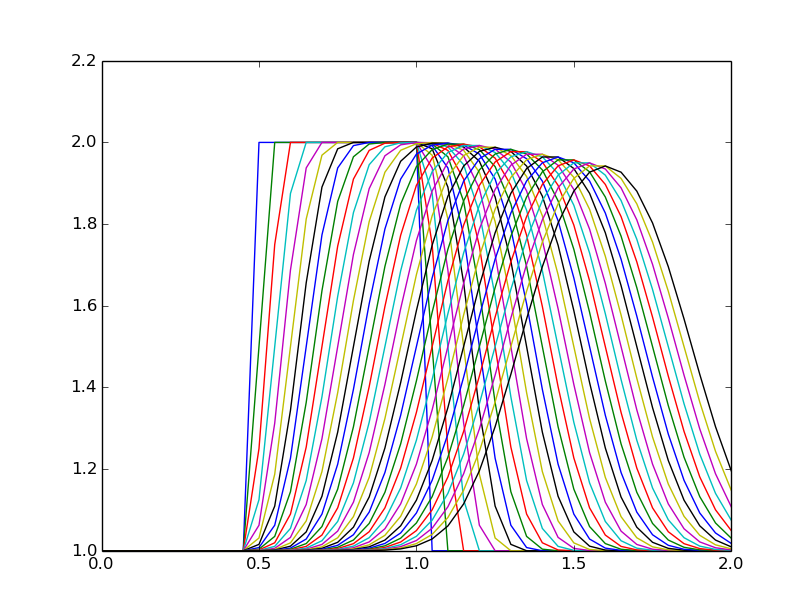
\includegraphics[scale=0.8]{num_diff.png}
	\label{fig:num_diff}
	\end{figure}

Figure \ref{fig:num_diff_fine_mesh} shows that making a finer spatial grid reduces the
numerical diffusion and it retains more of the initial condition's hat shape.

	\begin{figure}[num_diff_fine_mesh]
	\centering
	\caption{1-d linear convection only. Less false diffusion. Number of grid points nx=71}
	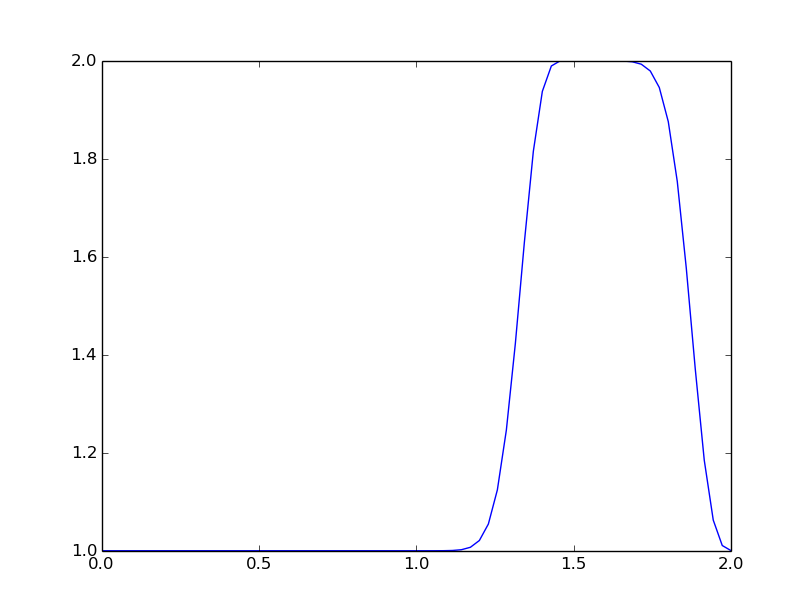
\includegraphics[scale=0.8]{better_hat.png}
	\label{fig:num_diff_fine_mesh}
	\end{figure}

	\begin{figure}[num_diff_finest_mesh]
	\centering
	\caption{1-d linear convection only. Hat mostly retained. Number of grid points nx=81}
	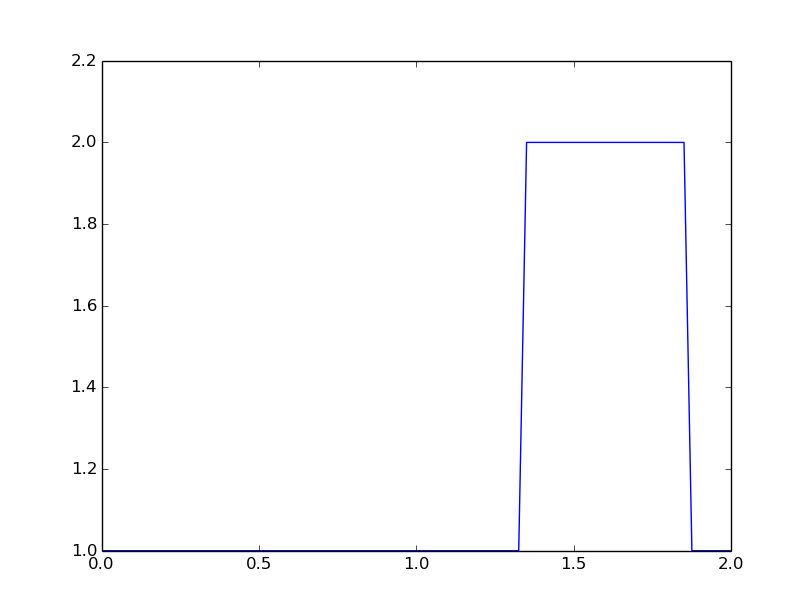
\includegraphics[scale=0.8]{keep_hat.png}
	\label{fig:num_diff_finest_mesh}
	\end{figure}

In figure \ref{fig:num_diff_finest_mesh} it appears that the hat has been retained by selecting
a fine mesh consisting of 81 points along the $x$-axis, but as soon as this is increased to
83 points, we see the artefacts that arise from not being constrained by the CFL condition
(figure \ref{fig:num_diff_too_fine}) and these effect grow quickly with the addition of only
a few more points to the spatial grid as seen in figure \ref{fig:num_diff_too_fine_explode}.

	\begin{figure}[num_diff_too_fine]
	\centering
	\caption{1-d linear convection only. CFL condition broken. Number of grid points nx=83}
	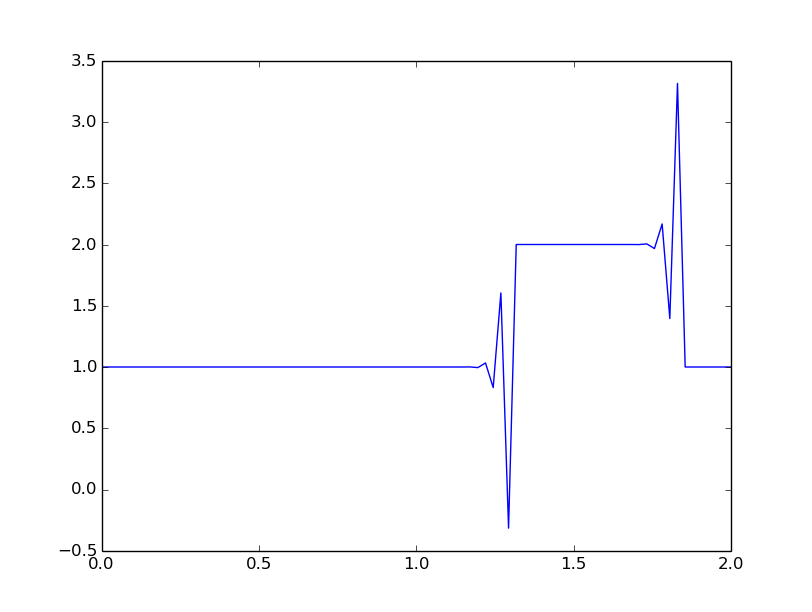
\includegraphics[scale=0.8]{cfl_broke.png}
	\label{fig:num_diff_too_fine}
	\end{figure}

	\begin{figure}[num_diff_too_fine_explode]
	\centering
	\caption{1-d linear convection only. Numerical artefacts dominate. nx=91}
	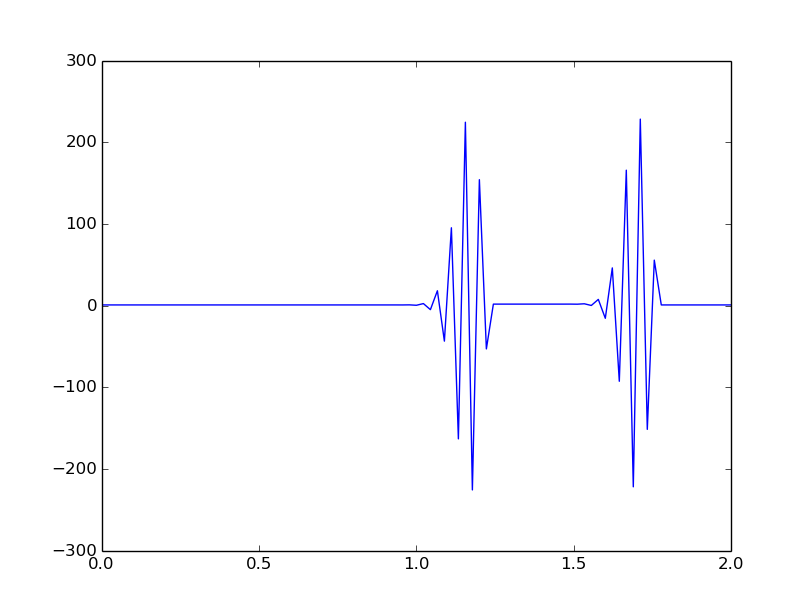
\includegraphics[scale=0.8]{cfl_explode.png}
	\label{fig:num_diff_too_fine_explode}
	\end{figure}

\subsubsection{Diffusion}
Moving into two dimensions. Here are some plots showing true physical diffusion.
The initial condition is a 2-d hat function shown in the first figure (\ref{fig:diff_0}),
an intermediate step (figure \ref{fig:diff_1}) is shown before it ends up at figure
\ref{fig:diff_final} after 50 timesteps. Large spatial grid (31 by 31) was chosen
for visualization purposes. Script used: \texttt{diffusion\_2d.py}

	\begin{figure}[diff_0]
	\centering
	\caption{2-d diffusion: Initial condition}
	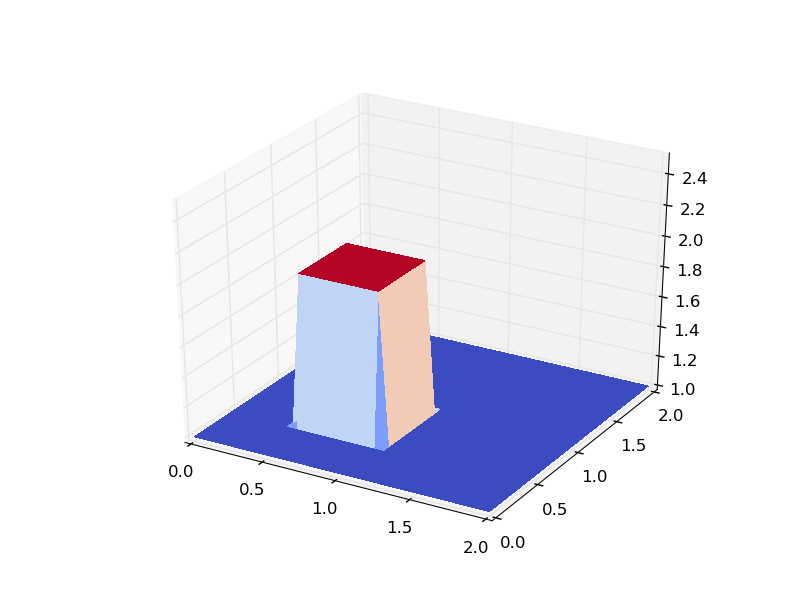
\includegraphics[scale=0.8]{diff_0.png}
	\label{fig:diff_0}
	\end{figure}

	\begin{figure}[diff_1]
	\centering
	\caption{2-d diffusion: Intermediate step (10 steps later)}
	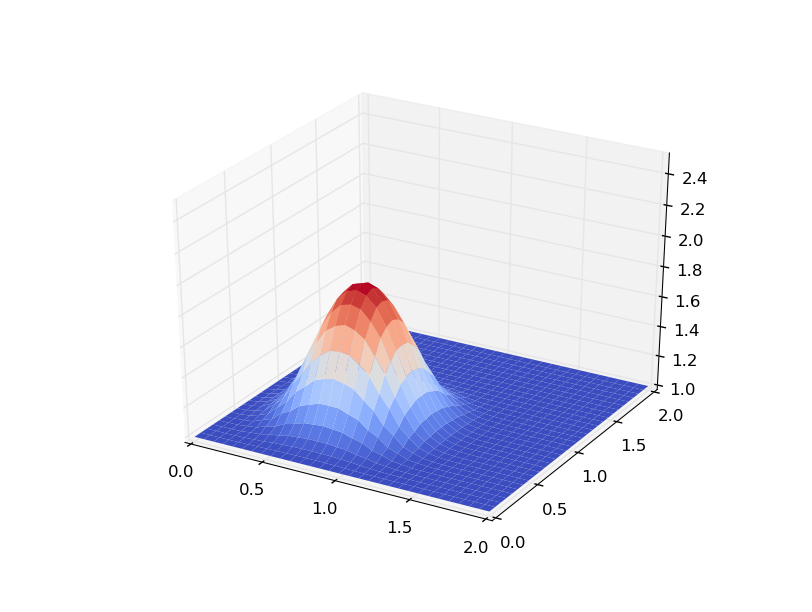
\includegraphics[scale=0.8]{diff_1.png}
	\label{fig:diff_1}
	\end{figure}
	
	\begin{figure}[diff_final]
	\centering
	\caption{2-d diffusion: Final step (50 steps after initial)}
	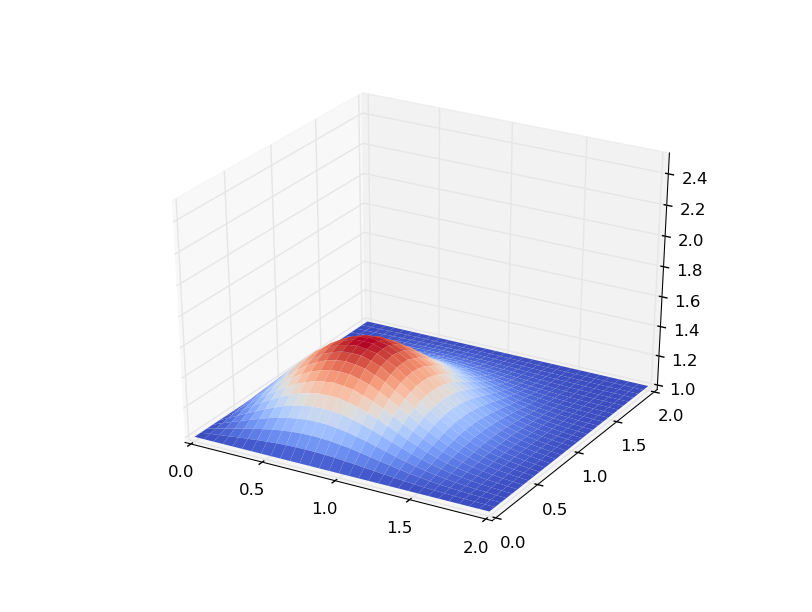
\includegraphics[scale=0.8]{diff_final.png}
	\label{fig:diff_final}
	\end{figure}


\subsubsection{Burgers}
w/w/o shocks
\subsubsection{Poisson}
\subsubsection{Navier-Stokes cavity flow}
\subsubsection{Navier-Stokes channel flow}




\section*{References}

\end{document}
